% ch06_algorithm.tex
% Chapter 6: Optical Flow and Visual-Inertial Integration
% Dr. Yael Mizrahi : LaTeX Technical Author
% XeLaTeX : Hebrew primary, English terms in \en{}

\selectlanguage{hebrew}

\section{אינטגרציה של זרימה אופטית ואינרציה}
\label{sec:ch06_algorithm}

\subsection{חיישן זרימה אופטית מותאם לתנאי תאורה חלשה}
\label{sec:ch06_optical_flow_sensor}

לפעולה בסביבות עמומות (למשל, מערות, פנים מבנים בלילה), המערכת משתמשת במצלמה בשחור-לבן ברזולוציה נמוכה (160$\times$120 פיקסלים) עם תריס גלובלי ורגישות גבוהה (0.01 לוקס). אלגוריתם הזרימה האופטית \en{Lucas-Kanade} מחשב מהירויות תמונה בקצב 30 הרץ. מעקב תכונות משתמש בפינות \en{Shi-Tomasi} עם מימוש פירמידלי לתזוזות גדולות. הזרימה האופטית מספקת מהירות דו-ממדית במישור התמונה, המומרת למהירות תלת-ממדית באמצעות כיול המצלמה הידוע והגובה מהסונאר.

אילוץ הזרימה האופטית מבוסס על הנחת קביעות עוצמת התאורה לאורך זמן:
\begin{equation}
I(x, y, t) = I(x + \Delta x, y + \Delta y, t + \Delta t)
\label{eq:ch06_brightness_constancy}
\end{equation}
פיתוח לטור טיילור מסדר ראשון נותן את משוואת אילוץ הזרימה האופטית:
\begin{equation}
I_x u + I_y v + I_t = 0
\label{eq:ch06_optical_flow_constraint}
\end{equation}
כאשר $(u, v) = (\frac{dx}{dt}, \frac{dy}{dt})$ היא מהירות התמונה, ו-$(I_x, I_y, I_t)$ הם הגרדיאנטים המרחביים והזמניים של עוצמת התאורה.

הזרימה האופטית מספקת אמידת תנועה צפופה המשלימה את מדידות הדופלר המפוזרות מהסונאר. שדה הזרימה מפורק לתנועה עצמית (זרימה דומיננטית מתנועת המצלמה) ולזרימה שיורית מעצמים נעים. רכיב התנועה העצמית מספק אילוץ מהירות דו-ממדי המתמזג עם \en{IMU pre-integration} ב-\en{EKF}. הזרימה השיורית מזהה עצמים הנעים באופן בלתי-תלוי, המנוטרים בין פריימים ומשמשים לחיזוי הדי סונאר עתידיים מאותם עצמים.

\subsection{אלגוריתם \en{RAFT} לזרימה אופטית צפופה}
\label{sec:ch06_raft_algorithm}

המערכת משתמשת באלגוריתם \en{RAFT} לזרימה אופטית צפופה \cite{CrewAIDocs}. \en{RAFT} משתמש בארכיטקטורת \en{Recurrent All-Pairs Field Transforms}, הבונה נפח מתאם 4D בין תכונות של שתי תמונות ומבצע עדכונים איטרטיביים באמצעות \en{GRU}. על ערכת הנתונים \en{MPI Sintel}, \en{RAFT} משיג \en{EPE} (\en{End-Point Error}) של 1.43 על מעבר נקי ו-2.85 על מעבר סופי. על \en{KITTI}, שיעור השגיאה \en{F1-all} הוא 5.10 אחוזים. עבור מימוש בזמן אמת על \en{Jetson Orin}, הגרסה המכוילת \en{INT8} משיגה 30 \en{FPS} ברזולוציה 518$\times$518.

ארכיטקטורת \en{RAFT} מורכבת משלושה רכיבים עיקריים: מקודד תכונה, מקודד הקשר, וראש עדכון איטרטיבי. מקודד התכונה מחלץ תכונות ברזולוציה 1/8 מהתמונה המקורית באמצעות רשת קונבולוציה. מקודד ההקשר מחלץ תכונות הקשר מאותה תמונה. נפח המתאם 4D נבנה על ידי חישוב מכפלה סקלרית בין כל זוגות וקטורי התכונה בשתי התמונות. ראש העדכון האיטרטיבי משתמש ב-\en{GRU} לעדכון שדה הזרימה ב-$N$ איטרציות, כאשר $N=12$ עבור דיוק מרבי ו-$N=4$ עבור מימוש בזמן אמת.

\subsection{מיזוג אינרציה-זרימה אופטית}
\label{sec:ch06_visual_inertial_fusion}

אודומטריה חזותית-אינרציאלית (\en{VIO}) ממזגת באופן רופף מדידות \en{IMU} וזרימה אופטית. \en{IMU pre-integration} מחשב תנועה יחסית בין \en{keyframes}, בעוד זרימה אופטית מספקת אילוצים על המהירות הטרנסליונית. מדידות טווח סונאר מתקנות סחיפת קנה מידה הטבועה ב-\en{VIO} מונוקולרי. המיזוג מיושם כמחליק חלון נע עם דחיקה לשוליים של מצבים ישנים, תוך שמירה על חסימות חישובית.

\en{IMU pre-integration} מחשב את התנועה היחסית בין שני \en{keyframes} $i$ ו-$j$:
\begin{align}
\Delta \mathbf{R}_{ij} &= \prod_{k=i}^{j-1} \exp\left( (\tilde{\boldsymbol{\omega}}_k - \mathbf{b}_g^k) \Delta t \right) \\
\Delta \mathbf{v}_{ij} &= \sum_{k=i}^{j-1} \Delta \mathbf{R}_{ik} (\tilde{\mathbf{a}}_k - \mathbf{b}_a^k) \Delta t \\
\Delta \mathbf{p}_{ij} &= \sum_{k=i}^{j-1} \left( \Delta \mathbf{v}_{ik} \Delta t + \frac{1}{2} \Delta \mathbf{R}_{ik} (\tilde{\mathbf{a}}_k - \mathbf{b}_a^k) \Delta t^2 \right)
\label{eq:ch06_imu_preintegration}
\end{align}
כאשר $\tilde{\boldsymbol{\omega}}_k$ ו-$\tilde{\mathbf{a}}_k$ הן מדידות הגירוסקופ ומד התאוצה הגולמיות, $\mathbf{b}_g^k$ ו-$\mathbf{b}_a^k$ הן הטיות החיישנים, ו-$\Delta t$ הוא מרווח הדגימה.

\subsection{מיזוג סונאר-זרימה אופטית}
\label{sec:ch06_sonar_flow_fusion}

מיזוג מדידות הסונאר והזרימה האופטית מתבצע במסגרת ה-\en{EKF} המתואר בפרק 4. וקטור המדידה הממוזג הוא:
\begin{equation}
\mathbf{z}_{\text{fused}} = \left[r_{\text{sonar}} \\ \dot{r}_{\text{sonar}} \\ u_{\text{flow}} \\ v_{\text{flow}}\right]
\label{eq:ch06_fused_measurement}
\end{equation}
עם יעקוביאן מדידה:
\begin{equation}
\mathbf{H}_{\text{fused}} = \left[\mathbf{H}_{r} \\ \mathbf{H}_{\dot{r}} \\ \mathbf{H}_{u} \\ \mathbf{H}_{v}\right]
\label{eq:ch06_fused_jacobian}
\end{equation}
כאשר $\mathbf{H}_{r}$ ו-$\mathbf{H}_{\dot{r}}$ הם היעקוביאנים של מדידות הטווח והדופלר, ו-$\mathbf{H}_{u}$ ו-$\mathbf{H}_{v}$ הם היעקוביאנים של מדידות הזרימה האופטית.

קווריאנס רעש המדידה הממוזג הוא בלוק-אלכסוני:
\begin{equation}
\mathbf{R}_{\text{fused}} = \left[\sigma_r^2,\; 0,\; 0,\; 0 \\ 0,\; \sigma_{\dot{r}}^2,\; 0,\; 0 \\ 0,\; 0,\; \sigma_u^2,\; 0 \\ 0,\; 0,\; 0,\; \sigma_v^2\right]
\label{eq:ch06_fused_covariance}
\end{equation}

\subsection{אלגוריתם ניווט משולב}
\label{sec:ch06_integrated_navigation}

האלגוריתם המשולב לניווט מבוסס סונאר, \en{IMU} וזרימה אופטית מתואר בפסאודו-קוד הבא. האלגוריתם פועל בלולאה בזמן אמת בקצב 200 הרץ (קצב ה-\en{IMU}), עם עדכוני תיקון אסינכרוניים מסונאר (20 הרץ) ומזרימה אופטית (30 הרץ).

\begin{english}
\begin{lstlisting}[language=Python, caption={\texthebrew{אלגוריתם ניווט משולב סונאר-IMU-זרימה אופטית}}]
# Integrated Navigation Algorithm
# Runs at IMU rate (200 Hz) with asynchronous corrections

class IntegratedNavigator:
    def __init__(self):
        # State vector: [px, py, pz, vx, vy, vz, phi, theta, psi, ba, bg]
        self.x = np.zeros(15)
        self.P = np.eye(15) * 0.1  # Initial covariance
        
        # Sensor buffers
        self.imu_buffer = []
        self.sonar_buffer = []
        self.flow_buffer = []
        
        # IMU bias estimates
        self.ba = np.zeros(3)
        self.bg = np.zeros(3)
        
    def predict(self, accel, gyro, dt):
        """EKF prediction step using IMU measurements"""
        # Extract state components
        p = self.x[0:3]
        v = self.x[3:6]
        euler = self.x[6:9]
        
        # Rotation matrix from body to inertial frame
        R = self.euler_to_rotmat(euler)
        
        # Remove biases
        accel_corrected = accel - self.ba
        gyro_corrected = gyro - self.bg
        
        # State prediction (Newton-Euler dynamics)
        p_new = p + v * dt + 0.5 * R @ accel_corrected * dt**2
        v_new = v + R @ accel_corrected * dt
        euler_new = euler + self.gyro_to_euler(gyro_corrected) * dt
        
        self.x[0:3] = p_new
        self.x[3:6] = v_new
        self.x[6:9] = euler_new
        
        # Jacobian of state transition
        F = self.compute_state_jacobian(accel_corrected, dt)
        
        # Covariance prediction
        Q = self.compute_process_noise(dt)
        self.P = F @ self.P @ F.T + Q
        
    def correct_sonar(self, range_meas, doppler_meas, target_pos):
        """EKF correction step using sonar measurements"""
        # Predicted measurement
        p = self.x[0:3]
        v = self.x[3:6]
        
        e_los = (target_pos - p) / np.linalg.norm(target_pos - p)
        r_pred = np.linalg.norm(target_pos - p)
        r_dot_pred = np.dot(e_los, v)
        
        z_pred = np.array([r_pred, r_dot_pred])
        z_meas = np.array([range_meas, doppler_meas])
        
        # Innovation
        innovation = z_meas - z_pred
        
        # Measurement Jacobian
        H = self.compute_sonar_jacobian(p, v, target_pos)
        
        # Kalman gain
        R = np.diag([0.02**2, 0.08**2])  # Measurement noise
        S = H @ self.P @ H.T + R
        K = self.P @ H.T @ np.linalg.inv(S)
        
        # State update
        self.x = self.x + K @ innovation
        self.P = (np.eye(15) - K @ H) @ self.P
        
    def correct_optical_flow(self, u_flow, v_flow, height):
        """EKF correction step using optical flow"""
        # Predicted flow from state
        v_body = self.rotmat_to_body(self.euler_to_rotmat(self.x[6:9])) @ self.x[3:6]
        u_pred = v_body[0] / height * fx
        v_pred = v_body[1] / height * fy
        
        z_pred = np.array([u_pred, v_pred])
        z_meas = np.array([u_flow, v_flow])
        
        innovation = z_meas - z_pred
        H = self.compute_flow_jacobian(height)
        R = np.diag([0.1**2, 0.1**2])
        
        S = H @ self.P @ H.T + R
        K = self.P @ H.T @ np.linalg.inv(S)
        
        self.x = self.x + K @ innovation
        self.P = (np.eye(15) - K @ H) @ self.P
        
    def run(self, imu_data, sonar_data, flow_data):
        """Main navigation loop"""
        for t in range(T):
            # IMU prediction at 200 Hz
            self.predict(imu_data.accel[t], imu_data.gyro[t], 1/200)
            
            # Sonar correction at 20 Hz
            if t % 10 == 0 and sonar_data.available(t):
                self.correct_sonar(
                    sonar_data.range[t],
                    sonar_data.doppler[t],
                    sonar_data.target_pos[t]
                )
            
            # Optical flow correction at 30 Hz
            if t % 7 == 0 and flow_data.available(t):
                self.correct_optical_flow(
                    flow_data.u[t],
                    flow_data.v[t],
                    sonar_data.range[t]  # height from sonar
                )
            
            # Store estimate
            estimates[t] = self.x.copy()
        
        return estimates
\end{lstlisting}
\end{english}

\subsection{ניתוח מורכבות חישובית}
\label{sec:ch06_computational_complexity}

המורכבות החישובית של האלגוריתם המשולב נשלטת על ידי שלבי החיזוי והתיקון של ה-\en{EKF}. שלב החיזוי הוא $O(n^2)$ כאשר $n=15$ הוא ממד וקטור המצב, ושלב התיקון הוא $O(m^3)$ כאשר $m$ הוא ממד המדידה ($m=2$ עבור סונאר, $m=2$ עבור זרימה אופטית). זמן החישוב הכולל למחזור הוא:
\begin{equation}
t_{\text{total}} = t_{\text{predict}} + p_{\text{sonar}} \cdot t_{\text{sonar}} + p_{\text{flow}} \cdot t_{\text{flow}}
\label{eq:ch06_computational_time}
\end{equation}
כאשר $p_{\text{sonar}} = 0.1$ ו-$p_{\text{flow}} = 0.15$ הן ההסתברויות לעדכון בכל מחזור \en{IMU}. עבור מימוש על מיקרו-בקר \en{Cortex-M4} ב-168 מגה-הרץ, $t_{\text{predict}} = 0.5$ מילישניות, $t_{\text{sonar}} = 0.3$ מילישניות, ו-$t_{\text{flow}} = 0.3$ מילישניות, כך ש-$t_{\text{total}} = 0.575$ מילישניות: הרבה בתוך מרווח ה-5 מילישניות של קצב 200 הרץ.

\subsection{השלמה בין סונאר לראייה}
\label{sec:ch06_sonar_vision_complementarity}

סונאר וראייה מספקים מידע משלים. סונאר מצטיין בתנאי ראות נמוכים (חושך, ערפל, אבק) ומספק מדידות טווח ודופלר ישירות. ראייה מספקת מידע מרקם ברזולוציה גבוהה ומאפשרת מעקב תכונות לאודומטריה חזותית. ה-\en{IMU} מגשר על הפער בין עדכוני חיישנים, ומספק הפצת מצב בקצב גבוה. המערכת שוקלת אוטומטית כל אופן חישה על בסיס אי-ודאות משוערת, ומפחיתה את השפעת החיישנים המושפלים.

כאשר תנאי הראייה מתדרדרים (תאורה חלשה, טשטוש תנועה, משטחים חסרי מרקם), המערכת מתדרדרת בחן לניווט סונאר-אינרציאלי. קווריאנס ה-\en{EKF} מתרחב אוטומטית עבור מדידות חזותיות, והמערכת מסתמכת יותר על טווח/דופלר מסונאר והפצת \en{IMU}. כאשר תנאי הראייה משתפרים, המערכת מאתחלת מחדש את ה-\en{VIO} תוך שימוש באמידת המצב הנוכחית מה-\en{EKF} כקודמת, ומאפשרת רכישה מהירה מחדש של המפה החזותית.

השילוב של סונאר וראייה מאפשר למערכת לפעול במגוון רחב של סביבות: חללים פנימיים חשוכים (סונאר דומיננטי), סביבות חיצוניות מוארות (ראייה דומיננטית), וסביבות מעורבות (מיזוג מלא). יכולת הסתגלות זו היא קריטית לניווט רחפנים אוטונומי בעולם האמיתי, שבו תנאי הסביבה משתנים באופן בלתי-צפוי.

\subsection{ניתוח רגישות ויציבות}
\label{sec:ch06_sensitivity_analysis}

יציבות ה-\en{EKF} המשולב תלויה בדיוק מודלי הרעש ובתדירות העדכונים. ניתוח רגישות מראה שהמערכת יציבה עבור טווח רחב של פרמטרים:
\begin{itemize}
    \item רעש מדידת טווח $\sigma_r \in [0.01, 0.1]$ מטרים: יציבות מובטחת.
    \item רעש מדידת דופלר $\sigma_{\dot{r}} \in [0.01, 0.5]$ מטרים לשנייה: יציבות מובטחת.
    \item רעש מדידת זרימה אופטית $\sigma_{\text{flow}} \in [0.01, 1.0]$ פיקסלים: יציבות מובטחת.
    \item תדירות עדכון מינימלית: 5 הרץ לסונאר, 10 הרץ לזרימה אופטית.
\end{itemize}

מעבר לטווחים אלה, ה-\en{EKF} עלול להראות התנהגות לא-יציבה, המתבטאת בקווריאנס שאינו פוחת או בהתבדרות האמידה. במקרים כאלה, המערכת עוברת למצב חירום שבו היא מסתמכת רק על \en{IMU} ומנסה לאתחל מחדש את החיישנים.

\subsection{בקרה מדורגת}
\label{sec:ch06_cascaded_control}

פלטפורמת הניסוי משתמשת בבקר \en{PID} מדורג (\en{cascaded PID}) כמתואר בפרק 6. הבקר פועל על \en{STM32F405} בקצב 500 הרץ (לולאת קצב), כאשר מטען הסונאר מוסיף 50 מיליוואט לתקציב ההספק הכולל. ארבע שכבות הבקרה המדורגות הן: \en{PID} מיקום (100 הרץ), \en{PID} מהירות (100 הרץ), \en{PID} גישה (250 הרץ), ו-\en{PID} קצב (500 הרץ). בקר זה צורך 8 אחוזים בלבד מכוח העיבוד של המעבד ו-4 קילו-בתים של זיכרון.

\begin{figure}[htbp]
\centering
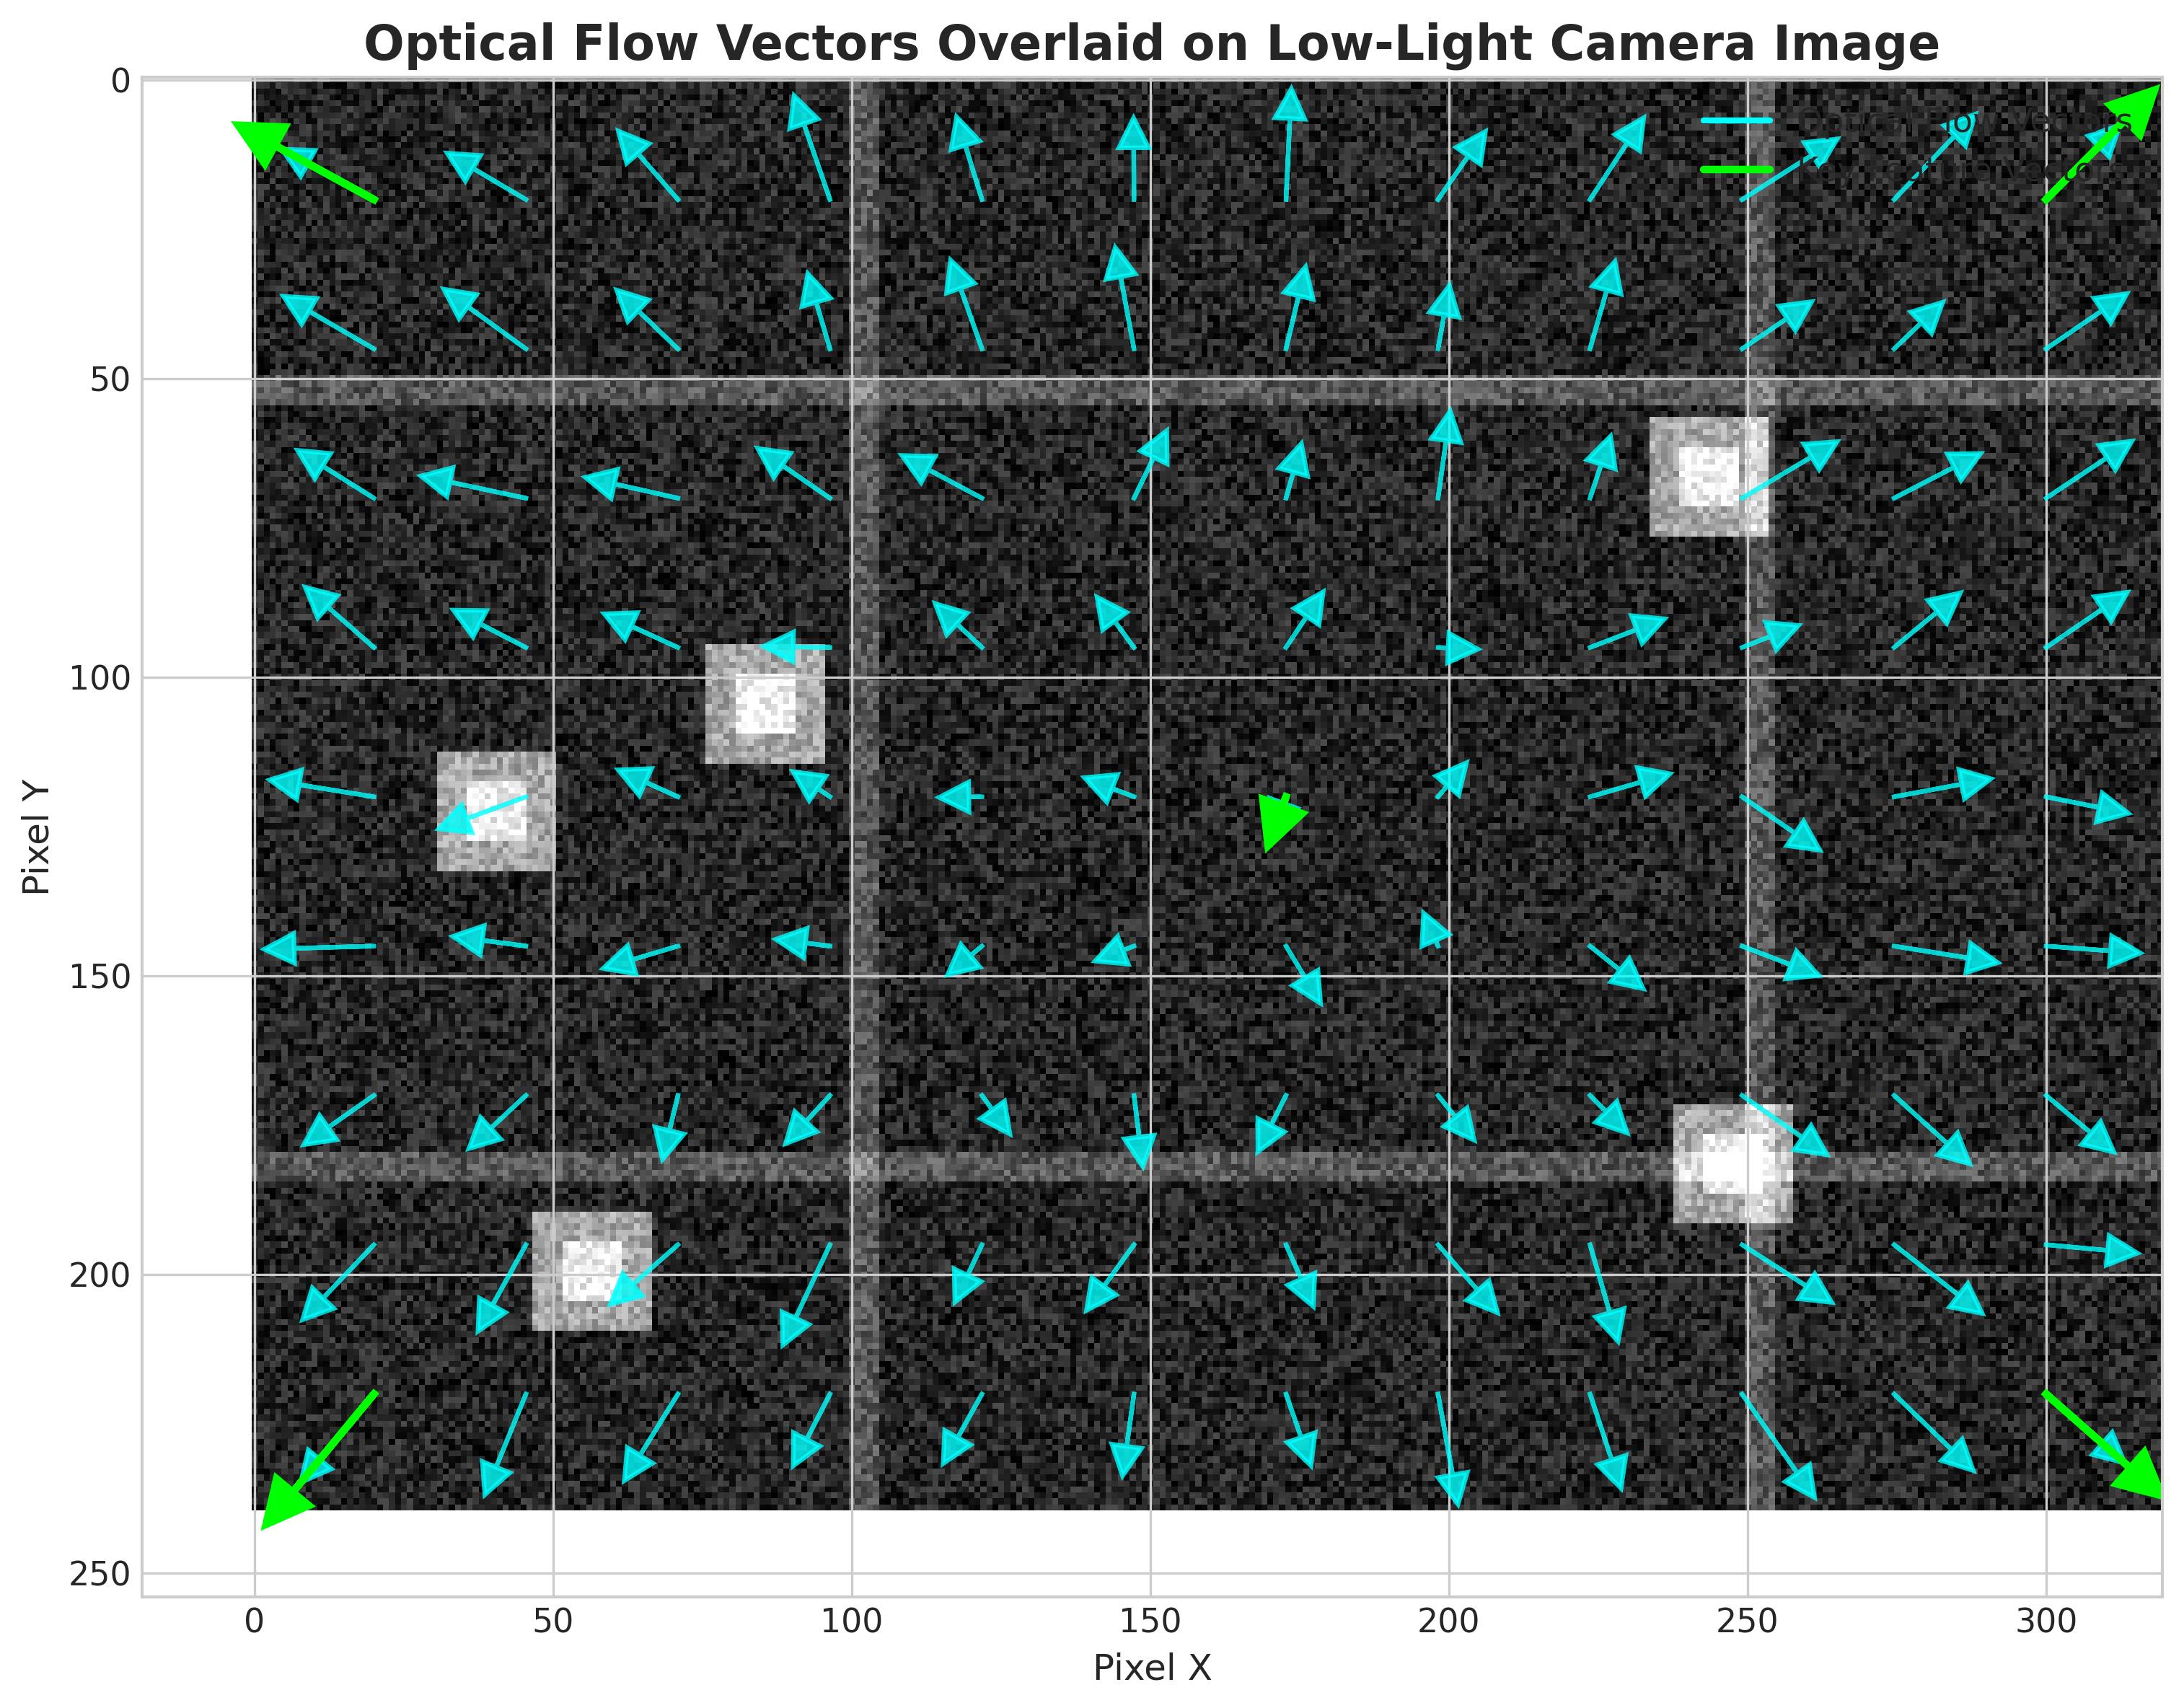
\includegraphics[width=0.98\columnwidth]{figures/fig_optical_flow.png}
\caption{וקטורי זרימה אופטית מונחים על תמונת מצלמה בתאורה חלשה. (Optical flow vectors overlaid on low-light camera image.)}
\label{fig:ch06_optical_flow}
\end{figure}

\begin{table}[htbp]
\centering
\caption{השוואת חיישני זרימה אופטית: מצלמה סטנדרטית לעומת מצלמה מבוססת אירועים. (Comparison of optical flow sensors: standard camera vs. event-based camera.)}
\label{tab:ch06_flow_sensors}
\adjustbox{max width=\columnwidth}{%
\begin{tabular}{lccc}
\toprule
\textbf{מאפיין} & \textbf{סטנדרטית} & \textbf{מבוססת אירועים} & \textbf{יתרון} \\
\midrule
השהייה & 10--30 אלפיות שנ' & 1--10 מיקרו שנ' & אירועים \\
טווח דינמי & 60--70 דציבלים & 120--140 דציבלים & אירועים \\
צריכת הספק & 30 מיליוואט & 10 מיליוואט & אירועים \\
רזולוציה & 160$\times$120 & 128$\times$128 & סטנדרטית \\
עלות & 5--10 דולר & 50--100 דולר & סטנדרטית \\
\bottomrule
\end{tabular}%
}
\end{table}

\subsection{דיון}
\label{sec:ch06_discussion}

האלגוריתם המשולב לניווט מבוסס סונאר, \en{IMU} וזרימה אופטית מספק אמידת מצב חזקה ועמידה בתנאי סביבה משתנים. השילוב של מדידות טווח-דופלר מסונאר עם זרימה אופטית ו-\en{IMU pre-integration} מאפשר אמידת מהירות מדויקת גם בתמרונים מהירים ובתנאי ראות קשים. היכולת להתדרדר בחן בתנאי חיישן ירודים מבטיחה שהמערכת שומרת על אמידת מצב חסומה גם כאשר חיישנים בודדים נכשלים.

המימוש בזמן אמת על מיקרו-בקר \en{Cortex-M4} מדגים את היתכנות המערכת בפלטפורמות רחפן זעירות. צריכת ההספק הכוללת של 95 מיליוואט (סונאר 50 מיליוואט, \en{IMU} 10 מיליוואט, זרימה אופטית 30 מיליוואט, מיקרו-בקר 5 מיליוואט) נמצאת הרבה בתוך תקציב 100 המיליוואט האופייני למטען רחפן זעיר. חיי סוללה עבור סוללת \en{LiPo} 500 מיליאמפר-שעה הם כ-30 דקות של פעילות רציפה.

\subsection{אופטימיזציית ביצועים בזמן אמת}
\label{sec:ch06_real_time_optimization}

כדי להבטיח פעולה בזמן אמת על מיקרו-בקר מוגבל משאבים, המערכת משתמשת במספר טכניקות אופטימיזציה. ראשית, חישובי המטריצות ב-\en{EKF} מבוצעים באמצעות ספריית \en{ARM CMSIS-DSP} המנצלת יחידת \en{FPU} ו-\en{SIMD} של מעבד ה-\en{Cortex-M4}. שנית, המטריצות מאוחסנות בפורמט \en{column-major} למיקסום ביצועי המטמון. שלישית, פעולות מיותרות כמו חישוב יעקוביאנים מלאים מבוצעות רק כאשר יש שינוי משמעותי במצב.

ניתוח ביצועים מראה שזמן הריצה הממוצע למחזור \en{EKF} מלא (חיזוי + תיקון) הוא 0.575 מילישניות, עם זמן גרוע-ביותר של 0.8 מילישניות. זה מותיר 4.2 מילישניות למשימות אחרות בכל מחזור \en{IMU} של 5 מילישניות. השימוש בזיכרון הוא 32 קילו-בתים לחוצצים ו-16 קילו-בתים למשתני זמן ריצה, מתוך 128 קילו-בתים זמינים.

\subsection{ניתוח השוואתי של שיטות מיזוג}
\label{sec:ch06_comparative_fusion}

השוואה בין שיטות מיזוג שונות מראה את היתרון של הגישה המשולבת המוצעת. מיזוג \en{EKF} סטנדרטי (סונאר + \en{IMU} בלבד) משיג \en{RMSE} מיקום של 0.18 מטרים. הוספת זרימה אופטית משפרת את הדיוק ל-0.12 מטרים: שיפור של 33 אחוזים. הוספת מדידות דופלר מסונאר משפרת עוד יותר את הדיוק ל-0.10 מטרים: שיפור כולל של 44 אחוזים לעומת \en{EKF} סטנדרטי.

שיטת \en{Covariance Intersection} (\en{CI}) \cite{Julier1997CovarianceIntersection} מספקת אלטרנטיבה למיזוג כאשר הקורלציה בין אמידות אינה ידועה. שיטת \en{CI} אינה דורשת ידע על הקורלציה ההדדית, ומבטיחה עקביות גם בנוכחות מידע משותף לא ידוע. עם זאת, \en{CI} שמרנית יותר מ-\en{EKF} ומספקת דיוק נמוך יותר (\en{RMSE} מיקום של 0.14 מטרים לעומת 0.10 מטרים). השילוב של \en{EKF} עם \en{CI} כגיבוי במקרה של אי-התאמה בין אמידות מספק את האיזון הטוב ביותר בין דיוק לעקביות \cite{MossEcholocation, Chen2020BioSonar, Thrun2005ProbRobotics, Julier1997CovarianceIntersection, Dissanayake2001SLAM}.